\section{扰动分析}
\label{sec:ls-perturbation}
\label{sec:linear-algebra-stability}
\label{sec:matrix-analysis-conditioning-perturbation}

前面各章在精确输入上建立了运算、求解与逼近。本节固定一个任务，回答一个更实际的问题：
交给算法的数据与理想输入相差一点时，答案会相差多少。\term{扰动}（perturbation）指
允许范围内的输入增量，扰动分析不改变任务本身，只测量输入增量被放大多少。先在
\ref{sec:ls-perturbation-conditioning}统一误差尺度与条件数，再依次估计基本运算、
方程解、最小二乘、谱值与子空间、矩阵函数的响应，最后把问题本身的敏感度与算法的
舍入误差分开（\ref{sec:ls-numerical-stability}）。每个结论都要写清所用范数、允许
改变的分量、秩或谱隙条件以及定义域边界；没有这些条件的“误差小”没有意义。

\subsection{扰动与条件数}
\label{sec:ls-perturbation-conditioning}

\subsubsection{输入、输出与误差}

\paragraph{固定运算与输入输出}

扰动分析的第一步是把任务固定下来：给定映射 $F$、理想输入 $\bm z$ 和明确的输出
$F(\bm z)$，再问 $\bm z$ 改变后 $F(\bm z)$ 改变多少。这里只改变数据，不更换算法；
“算法算错了”是另一项误差，在\ref{sec:ls-numerical-stability}节单独处理。任务不同，
比较的输出也不同：求逆比较逆矩阵，解方程比较解向量，最小二乘要分别比较系数、拟合值
与残差，谱分解要分别比较谱值与子空间。先指定输出对象，后面的误差尺度才有附着点。

\paragraph{输入增量和输出增量}

设实际输入为 $\bm z+\Delta\bm z$，其中 $\Delta\bm z$ 是输入增量，输出增量定义为
\[
 \Delta\bm y=F(\bm z+\Delta\bm z)-F(\bm z).
\]
对线性任务 $F(\bm z)=\bm A\bm z$，输出增量就是 $\Delta\bm y=\bm A\,\Delta\bm z$，
与理想输入 $\bm z$ 本身无关；对非线性任务，$\Delta\bm y$ 还通过 $F$ 依赖 $\bm z$。
扰动分析只比较两个输出的差，不要求写出 $F$ 的完整表达式。

\paragraph{绝对误差与相对误差}

绝对误差直接取增量范数 $\lVert\Delta\bm z\rVert$、$\lVert\Delta\bm y\rVert$；当输入
与输出本身有尺度时，更常用\term{相对误差}（relative error）
\[
 \frac{\lVert\Delta\bm z\rVert}{\lVert\bm z\rVert},
 \qquad
 \frac{\lVert\Delta\bm y\rVert}{\lVert F(\bm z)\rVert}.
\]
相对误差对整体缩放不变：把所有数据乘以 $10^3$，绝对误差同步放大，相对误差不变，
因此它反映“变化占原有量的比例”。\term{绝对误差}（absolute error）则保留实际大小，
在输出接近零时必须使用。

\paragraph{零输入或零输出的尺度边界}

分母为零时相对误差没有定义：$\bm z=\bm0$ 时不能除以 $\lVert\bm z\rVert$，
$F(\bm z)=\bm0$ 时不能除以 $\lVert F(\bm z)\rVert$。此时报告绝对误差，或改用任务
指定的参考尺度（如矩阵范数 $\lVert\bm A\rVert$）。秩变化等不连续处也不能套用
“小输入产生小输出”的微分式判断，伪逆在秩改变处的跳变见\ref{sec:ls-ordinary-ls-sensitivity}。

\paragraph{范数选择与结构约束}

误差大小依赖所选范数，同一增量在 $\ell_1$、$\ell_2$、Frobenius 范数下数值不同，
比较前必须写明口径。还要写明允许改变哪些分量：只改右端、同时改矩阵与右端、要求
扰动矩阵保持对称，得到的敏感度不同。例如只允许右端变化的方程，与允许系数矩阵
一起变化的方程，不是同一个扰动问题。

\subsubsection{条件数}

\paragraph{有限增量的局部放大比}

对固定任务 $F$，输入增量 $\Delta\bm z$ 引起的输出增量 $\Delta\bm y$，其放大比为
$\lVert\Delta\bm y\rVert/\lVert\Delta\bm z\rVert$。扰动分析取足够小的允许增量，观察
这个比值在局部的上界；它是有限增量的比值，不预先使用导数。

\paragraph{允许扰动中的最坏方向}

输入增量可以朝任意允许方向取，敏感度由最坏方向决定：
\[
 \sup_{\Delta\bm z\neq0}
 \frac{\lVert F(\bm z+\Delta\bm z)-F(\bm z)\rVert}
      {\lVert\Delta\bm z\rVert}.
\]
对线性作用 $\bm x\mapsto\bm A\bm x$，这个上确界就是第~\ref{sec:ls-matrix-norms}节
建立的诱导范数 $\lVert\bm A\rVert$，在最大放大方向达到；它不描述某一个具体扰动，
而描述所有允许扰动中最不利的那个。

\paragraph{绝对条件数}

任务 $F$ 在 $\bm z$ 处的\term{绝对条件数}（absolute condition number）定义为
局部放大比的上确界；线性作用 $\bm A$ 的绝对条件数就是 $\lVert\bm A\rVert$。
绝对条件数带单位，随整体缩放改变，适合零输入或零输出的场合。

\paragraph{相对尺度与相对条件数}

把输入、输出都换成相对尺度，得到\term{相对条件数}（relative condition number）
\[
 \kappa_{\mathrm{rel}}(F;\bm z)
 =\sup_{\Delta\bm z\neq0}
 \frac{\lVert\Delta\bm y\rVert/\lVert F(\bm z)\rVert}
      {\lVert\Delta\bm z\rVert/\lVert\bm z\rVert}.
\]
对线性作用 $\bm x\mapsto\bm A\bm x$（$\bm x\neq\bm0$），
\[
 \kappa_{\mathrm{rel}}(\bm A;\bm x)
 =\frac{\lVert\bm A\rVert\,\lVert\bm x\rVert}{\lVert\bm A\bm x\rVert},
\]
它随方向变化：落在被压缩方向上的 $\bm x$ 放大比大，落在主伸缩方向上则小。

\paragraph{矩阵作用和求逆的不同敏感度}

对可逆方阵 $\bm A$，求逆任务 $\bm y\mapsto\bm A^{-1}\bm y$ 在所有方向上的最坏
相对条件数为
\begin{equation}
 \kappa(\bm A)=\lVert\bm A\rVert\,\lVert\bm A^{-1}\rVert,
 \label{eq:matrix-analysis-condition-number}
\end{equation}
它与作用任务在单个 $\bm x$ 处的相对条件数不是同一个量。欧氏范数下由SVD
（\ref{sec:ls-svd}）给出
\begin{equation}
 \kappa_2(\bm A)=\frac{\sigma_{\max}(\bm A)}{\sigma_{\min}(\bm A)}.
 \label{eq:matrix-analysis-spectral-condition-number}
\end{equation}
$\lVert\bm I\rVert=1$ 与次乘性保证 $\kappa(\bm A)\geq1$；正交矩阵 $\kappa_2=1$，
接近奇异时 $\sigma_{\min}\to0$，$\kappa_2$ 增大。同一个 $\bm A$，沿某个特定右端
作用可能很稳，求逆或反求系数却可能很敏感，因此矩阵没有一个包办所有任务的
“通用条件数”。

\begin{definition}[可逆矩阵的条件数]
\label{def:matrix-analysis-condition-number}
对同一向量范数诱导的矩阵范数，可逆方阵 $\bm A$ 的条件数为式
~\eqref{eq:matrix-analysis-condition-number}。它记录求逆任务的最坏相对放大，
不直接等于作用在某个具体右端上的放大比。
\end{definition}

\paragraph{条件数的适用范围与最坏界}

条件数是最坏方向上的上界，不是每个扰动都达到的倍数；它控制足够小的局部扰动，
有限扰动还要保留到奇异边界的余量（\ref{sec:ls-inverse-sensitivity}）。条件数
回答“一次输入增量被放大多少”，不回答反复作用的长期增长或衰减，后者属收敛分析。

\subsection{基本运算的敏感度}
\label{sec:ls-basic-operations-sensitivity}

本节用增量展开估计第~\ref{sec:ls-operations-summary}节各基本运算的响应，不重复
运算定义与计算教程。范数口径默认与输入输出一致，未注明处使用诱导范数或
Frobenius 范数。

\subsubsection{加法与乘法}

\paragraph{加减运算的增量恒等式}

两个输入分别改变：$(\bm x+\Delta\bm x)\pm(\bm y+\Delta\bm y)
-(\bm x\pm\bm y)=\Delta\bm x\pm\Delta\bm y$，故
\[
 \lVert\Delta(\bm x\pm\bm y)\rVert
 \leq\lVert\Delta\bm x\rVert+\lVert\Delta\bm y\rVert.
\]
加法本身不放大误差，两项误差按三角不等式相加；输出大小不进入这个绝对界。

\paragraph{输入抵消与相对误差}

当 $\bm x\approx-\bm y$ 时，理想输出 $\bm x+\bm y$ 很小，两项的绝对误差不变，
相对误差 $\lVert\Delta\bm x+\Delta\bm y\rVert/\lVert\bm x+\bm y\rVert$ 却被小分母
放大。例如 $x=1.0001$、$y=-1.0000$，各带 $5\times10^{-5}$ 的绝对误差，理想和为
$10^{-4}$，相对误差可达 $1$ 量级。抵消不是算法失误，而是小输出使相对尺度失效，
此时应报告绝对误差。

\paragraph{矩阵作用的输入增量}

系数矩阵固定、右端改变时，$\Delta(\bm A\bm x)=\bm A\,\Delta\bm x$，故
$\lVert\Delta(\bm A\bm x)\rVert\leq\lVert\bm A\rVert\lVert\Delta\bm x\rVert$。
正向作用的绝对放大由诱导范数控制，与 $\bm x$ 无关。

\paragraph{算子范数与最大放大方向}

最坏方向上 $\lVert\bm A\Delta\bm x\rVert/\lVert\Delta\bm x\rVert$ 达到
$\lVert\bm A\rVert$；欧氏范数下即最大奇异值 $\sigma_{\max}$。反方向
（由输出反求输入）才除以 $\sigma_{\min}$，那是求逆任务的事。

\paragraph{两侧矩阵扰动与交叉项}

两个因子都改变时，
\[
 (\bm A+\Delta\bm A)(\bm x+\Delta\bm x)-\bm A\bm x
 =\bm A\,\Delta\bm x+\Delta\bm A\,\bm x+\Delta\bm A\,\Delta\bm x.
\]
前两项分别是固定矩阵对另一侧增量的响应，最后一项是两个增量的乘积，在小扰动下
为二阶量。矩阵乘积同理：
$(\bm A+\bm E)(\bm B+\bm F)-\bm A\bm B
=\bm A\bm F+\bm E\bm B+\bm E\bm F$。

\paragraph{乘积误差的尺度与边界}

取相容范数，
\[
 \lVert(\bm A+\bm E)(\bm B+\bm F)-\bm A\bm B\rVert
 \leq\lVert\bm A\rVert\lVert\bm F\rVert
 +\lVert\bm E\rVert\lVert\bm B\rVert
 +\lVert\bm E\rVert\lVert\bm F\rVert.
\]
相对形式把各项除以 $\lVert\bm A\bm B\rVert$，大因子本身会放大另一侧的误差；
二阶项 $\lVert\bm E\rVert\lVert\bm F\rVert$ 在 $\lVert\bm E\rVert,\lVert\bm F\rVert$
足够小时可略去。逐项乘法（Hadamard）每个位置独立，误差按位置相乘，不跨位置求和。

\subsubsection{配对与度量}

\paragraph{内积的两侧增量}

$\langle\bm x,\bm y\rangle$ 两侧分别改变：
\[
 \Delta\langle\bm x,\bm y\rangle
 =\langle\Delta\bm x,\bm y\rangle+\langle\bm x,\Delta\bm y\rangle
 +\langle\Delta\bm x,\Delta\bm y\rangle.
\]
由 Cauchy--Schwarz（\ref{sec:ls-inner-products}），一阶项不超过
$\lVert\bm y\rVert\lVert\Delta\bm x\rVert
+\lVert\bm x\rVert\lVert\Delta\bm y\rVert$，末项为二阶。

\paragraph{近正交与小配对值}

理想内积 $\langle\bm x,\bm y\rangle\approx0$ 时，扰动项 $\langle\Delta\bm x,\bm y\rangle$
相对于近零的配对值可能很大，相对误差无意义。此时几何关系（是否正交）由投影分量
判断，配对数值本身只报告绝对变化。

\paragraph{权重变化与正定性保持}

加权配对 $\langle\bm M\bm x,\bm y\rangle$ 中加权矩阵 $\bm M$ 也改变。$\bm M$ 对称
正定时，若 $\lVert\bm M^{-1/2}\Delta\bm M\,\bm M^{-1/2}\rVert_2<1$，扰动后仍
正定：对任意 $\bm v$，
$\bm v^\top(\bm M+\Delta\bm M)\bm v
=\lVert\bm M^{1/2}\bm v\rVert^2
+\bm v^\top\Delta\bm M\bm v>0$。正定余量不足时先失去正定性，再谈配对误差。

\paragraph{加权配对的联合误差}

联合展开
\[
\Delta(\langle\bm M\bm x,\bm y\rangle)
=\langle\Delta\bm M\,\bm x,\bm y\rangle
+\langle\bm M\Delta\bm x,\bm y\rangle
+\langle\bm M\bm x,\Delta\bm y\rangle
+\text{二阶项},
\]
三项分别由加权矩阵、第一输入、第二输入的变化贡献，加权矩阵误差还乘以 $\lVert\bm x\rVert$，
大输入会放大加权矩阵误差。

\paragraph{范数的反三角不等式}

范数本身对输入扰动绝对稳定：由三角不等式的反向形式，
\[
 \big|\lVert\bm x+\Delta\bm x\rVert-\lVert\bm x\rVert\big|
 \leq\lVert\Delta\bm x\rVert.
\]
长度读数不会因为方向转动而剧烈变化；相对误差只在 $\bm x$ 接近零时需要小心。

\paragraph{距离的绝对界与相对尺度}

距离 $d(\bm x,\bm y)=\lVert\bm x-\bm y\rVert$ 满足
\[
 d(\bm x+\Delta\bm x,\bm y+\Delta\bm y)
 \leq d(\bm x,\bm y)+\lVert\Delta\bm x\rVert+\lVert\Delta\bm y\rVert.
\]
两点几乎重合时理想距离接近零，相对距离改用绝对距离或任务参考尺度报告。

\subsubsection{重排与张量运算}

\paragraph{重排与系数误差的对应}

转置、轴置换、reshape（\ref{sec:ls-reshaping}）只改变索引记录，不改动元素。
系数误差随位置一一对应搬到新数组，不产生新的求和或抵消，逐项范数误差原样保留。

\paragraph{保持的范数与改变的矩阵尺度}

置换保持 Frobenius 范数与逐项 $\ell_2$ 误差；但同一组元素从向量改成矩阵后，诱导
矩阵范数改变，因此“作为变换的放大能力”改变，尽管元素一个未动。重排不制造误差，
只改变后续口径下的尺度读数。

\paragraph{张量积的因子增量展开}

$(\bm A+\bm E)\otimes(\bm B+\bm F)-\bm A\otimes\bm B
=\bm E\otimes\bm B+\bm A\otimes\bm F+\bm E\otimes\bm F$。
张量积范数满足 $\lVert\bm A\otimes\bm B\rVert=\lVert\bm A\rVert\lVert\bm B\rVert$，
故一阶界为 $\lVert\bm E\rVert\lVert\bm B\rVert
+\lVert\bm A\rVert\lVert\bm F\rVert$。

\paragraph{Kronecker作用的放大界}

Kronecker 积作用在向量化矩阵上（\ref{sec:ls-kronecker-products}），
$\lVert(\bm A\otimes\bm B)\operatorname{vec}\bm X\rVert
\leq\lVert\bm A\rVert\lVert\bm B\rVert\lVert\bm X\rVert$；两侧因子的条件数
相乘进入放大，不能只看其中一个。

\paragraph{缩约求和中的权重传播}

缩约 $\sum_i x_i y_i$（\ref{sec:ls-tensor-contraction}）对每个因子分别线性，
但求和把多项误差累加：绝对误差不超过各项误差绝对值之和，项数越多累计越大。

\paragraph{抵消与输出相对误差}

求和中大小相近、符号相反的项抵消后输出很小，各项的累计绝对误差相对输出被放大；
迹（见下一小节）就是对角项的缩约，同样遵守这条边界。

\subsubsection{迹与行列式}

\paragraph{迹的增量与对角误差}

$\operatorname{tr}(\bm A+\bm E)-\operatorname{tr}\bm A
=\operatorname{tr}\bm E=\sum_i e_{i,i}$，故
$|\operatorname{tr}\bm E|\leq\sum_i|e_{i,i}|
\leq\sqrt r\,\lVert\bm E\rVert_{\mathrm F}$（$r$ 为阶数）。迹只读取对角项，
非对角误差不进入结果。

\paragraph{对角抵消与相对读取误差}

对角元素符号相反、大小相近时，理想迹接近零，对角误差之和相对迹被放大。迹是
标量读取量，矩阵本身可能完全正常，只是这个读数不适合用相对误差评价。

\paragraph{行列式的多线性增量展开}

行列式对每一列多线性（\ref{sec:ls-determinant-properties}）。把 $\bm A+\bm E$ 的
各列依次替换，一阶展开为
\[
 \det(\bm A+\bm E)-\det\bm A
 =\sum_{i=1}^d\det[\bm a_1,\dots,\bm e_i,\dots,\bm a_d]
 +O(\lVert\bm E\rVert^2),
\]
高阶项同时替换两列以上，是二阶及以上量。

\paragraph{单列变化与高阶交叉项}

只改第 $i$ 列时，差值等于该列余子式乘 $e_i$；多列同时改变产生交叉项。一阶界按
各列余子式求和估计，不把所有扰动塞进单一比值。

\paragraph{近奇异矩阵的体积敏感度}

$|\det\bm A|=\prod_i\sigma_i$（Gram 体积）。对角例子 $\bm A=\operatorname{diag}(1,\varepsilon)$，
$\det\bm A=\varepsilon$，第二对角元改变 $\delta\varepsilon$ 时相对变化为
$|\delta\varepsilon|/\varepsilon$；$\varepsilon\to0$ 时体积读数对微小变化
无限敏感，这是接近奇异的直接表现。

\paragraph{零行列式处的绝对误差}

$\det\bm A=0$ 时相对误差无定义，只报告绝对变化 $|\det(\bm A+\bm E)|$；
秩从 $0$ 变为非零属于不连续边界，不能用局部界外推。

\subsection{方程解的敏感度}
\label{sec:ls-equation-sensitivity}

\subsubsection{逆矩阵}
\label{sec:ls-inverse-sensitivity}
\label{sec:ch06-inverse-stability}

\paragraph{最小奇异值与输入下界}

$\bm A$ 可逆时，SVD（\ref{sec:ls-svd}）给出 $\lVert\bm A\bm x\rVert_2\geq\sigma_{\min}(\bm A)\lVert\bm x\rVert_2$，
因而 $\lVert\bm A^{-1}\rVert_2=1/\sigma_{\min}(\bm A)$。最小奇异值越小，逆对任意
输入的放大越大，这是求逆敏感度的根源。

\paragraph{扰动后的下界与可逆邻域}

设 $\bm B=\bm A+\bm E$。若 $\lVert\bm A^{-1}\bm E\rVert<1$，则 $\bm B$ 可逆：
假设 $\bm B\bm x=\bm0$，则 $\bm A\bm x=-\bm E\bm x$，左乘 $\bm A^{-1}$ 得
$\bm x=-\bm A^{-1}\bm E\bm x$，取范数有
$\lVert\bm x\rVert\leq\lVert\bm A^{-1}\bm E\rVert\lVert\bm x\rVert$，
与 $\bm x\neq\bm0$ 矛盾。这是有限增量的直接论证，不借助展开级数。

\paragraph{逆矩阵差的恒等式}

由 $\bm B\bm B^{-1}=\bm A\bm A^{-1}=\bm I$ 直接整理，
\begin{equation}
 \bm B^{-1}-\bm A^{-1}
 =-\bm B^{-1}\bm E\,\bm A^{-1},
 \label{eq:ch06-inverse-finite-perturbation}
\end{equation}
这是精确恒等式，不含高阶余项；差分被夹在两个逆之间。

\paragraph{逆差的绝对误差界}

从恒等式取范数，
$\lVert\bm B^{-1}-\bm A^{-1}\rVert
\leq\lVert\bm B^{-1}\rVert\lVert\bm E\rVert\lVert\bm A^{-1}\rVert$。
估计 $\bm B^{-1}$：由 $\bm B\bm x=\bm y$ 得
$\bm x=\bm A^{-1}(\bm y-\bm E\bm x)$，故
\[
 \lVert\bm x\rVert
 \leq\frac{\lVert\bm A^{-1}\rVert}{1-\lVert\bm A^{-1}\bm E\rVert}
 \lVert\bm y\rVert,
\]
即 $\lVert\bm B^{-1}\rVert
\leq\lVert\bm A^{-1}\rVert/(1-\lVert\bm A^{-1}\bm E\rVert)$。

\paragraph{相对误差与条件数}

代入恒等式，相对逆差满足
\[
 \frac{\lVert\bm B^{-1}-\bm A^{-1}\rVert}
      {\lVert\bm A^{-1}\rVert}
 \leq
 \frac{\kappa(\bm A)\,\lVert\bm E\rVert/\lVert\bm A\rVert}
      {1-\kappa(\bm A)\,\lVert\bm E\rVert/\lVert\bm A\rVert},
\]
分子是条件数乘相对扰动，分母保留到奇异边界的余量。

\paragraph{接近奇异边界的放大}

令 $\alpha=\kappa(\bm A)\lVert\bm E\rVert/\lVert\bm A\rVert$。$\alpha$ 越接近 $1$，
分母越小，逆差急剧放大；$\alpha\geq1$ 只表示本界失效、可逆性未被保证，
不等于 $\bm B$ 一定奇异。对角例子 $\bm A=\operatorname{diag}(1,\varepsilon)$，
$\kappa_2=1/\varepsilon$，相对扰动 $\delta$ 放大到 $\delta/(\varepsilon-\delta)$，
$\varepsilon\to0$ 时边界无限接近。

\subsubsection{线性方程}
\label{sec:ls-linear-system-sensitivity}

\paragraph{固定系数下的右端扰动}

$\bm A$ 固定、右端由 $\bm b$ 变为 $\bm b+\Delta\bm b$，由
$\bm A(\bm x+\Delta\bm x)=\bm b+\Delta\bm b$ 得 $\Delta\bm x=\bm A^{-1}\Delta\bm b$，
故
\[
 \lVert\Delta\bm x\rVert\leq\lVert\bm A^{-1}\rVert\lVert\Delta\bm b\rVert.
\]
绝对误差只受逆范数控制；相对形式为
\[
 \frac{\lVert\Delta\bm x\rVert}{\lVert\bm x\rVert}
 \leq\kappa(\bm A)\frac{\lVert\Delta\bm b\rVert}{\lVert\bm b\rVert}.
\]

\paragraph{奇异方向与解误差放大}

小奇异值方向把右端误差放大 $1/\sigma_{\min}$ 倍。两个 $2\times2$ 例子对照。
良态情形取 $\bm A_1=\begin{smallmatrix}2&0\\0&1\end{smallmatrix}$，
$\kappa_2=2$；右端由 $\bm b_1=(2,1)^\top$ 改为 $\bm b_1'=(2,1.01)^\top$，
解由 $(1,1)^\top$ 变为 $(1,1.01)^\top$：右端相对变化 $0.01/\sqrt5\approx0.00447$，
解的相对变化 $0.01/\sqrt2\approx0.00707$，放大比约 $1.58$，不超过 $\kappa_2=2$。
近平行情形取 $\bm A_2=\begin{smallmatrix}1&1\\0&\varepsilon\end{smallmatrix}$
（$\varepsilon>0$ 很小），两列接近同向，其最小奇异值约为 $\varepsilon/\sqrt2$、
$\kappa_2\approx2/\varepsilon$。取 $\varepsilon=10^{-2}$、右端 $\bm b=(1,0)^\top$，
解为 $\bm x=(1,0)^\top$；只把第二分量改动 $\eta=10^{-2}$ 得 $\bm b'=(1,\eta)^\top$，
由 $\varepsilon x_2=\eta$ 与 $x_1+x_2=1$ 得 $x_2=1$、$x_1=0$，解由 $(1,0)^\top$
跳到 $(0,1)^\top$：右端相对变化仅 $\eta=10^{-2}$，解的相对变化却为 $\sqrt2$，
放大比约 $\sqrt2/\eta\approx141$，与 $\kappa_2\approx2/\varepsilon=200$ 同量级。
系数矩阵接近平行的方向，其系数对观测误差高度敏感；两个例子都不含浮点误差，
差别完全来自问题本身。

\paragraph{系数和右端的联合扰动}

$\bm A+\bm E$、$\bm b+\Delta\bm b$ 同时改变，$\bm x+\Delta\bm x$ 满足
$(\bm A+\bm E)(\bm x+\Delta\bm x)=\bm b+\Delta\bm b$，减去理想方程
$\bm A\bm x=\bm b$，得到解差方程
\[
 \bm A\,\Delta\bm x=\Delta\bm b-\bm E\bm x-\bm E\Delta\bm x.
\]

\paragraph{解差方程与误差界}

把 $\bm E\Delta\bm x$ 移到左侧并整理，
\begin{equation}
 \frac{\lVert\Delta\bm x\rVert}{\lVert\bm x\rVert}
 \leq
 \frac{\kappa(\bm A)}{1-\kappa(\bm A)\lVert\bm E\rVert/\lVert\bm A\rVert}
 \left(
 \frac{\lVert\Delta\bm b\rVert}{\lVert\bm b\rVert}
 +\frac{\lVert\bm E\rVert}{\lVert\bm A\rVert}
 \right).
 \label{eq:matrix-analysis-linear-system-perturbation}
\end{equation}
右端扰动与系数扰动先相加，再被条件数放大，最后除以余量。

\paragraph{条件数和最坏相对误差}

式~\eqref{eq:matrix-analysis-linear-system-perturbation} 是最坏方向上的上界，
一般右端不一定达到；实际解差还与 $\Delta\bm b$、$\bm E$ 是否落在放大方向有关。
条件数给出天花板，不给出每个具体扰动的精确倍数。

\paragraph{有限扰动的可逆条件}

联合界成立的前提仍是 $\lVert\bm A^{-1}\bm E\rVert<1$；余量不足时先确认
$\bm A+\bm E$ 可逆，再谈解差。秩亏或近秩亏时唯一性本身不成立，界不存在。

\subsubsection{矩阵方程}
\label{sec:ls-matrix-equation-sensitivity}

\paragraph{矩阵方程上的线性算子}

把 $\bm Z$ 看作 Frobenius 空间中的向量，Sylvester 算子
$\mathcal L(\bm Z)=\bm A\bm Z+\bm Z\bm B$（\ref{def:matrix-analysis-sylvester-equation}）
是线性算子；其可逆条件 $\lambda_i(\bm A)+\lambda_j(\bm B)\neq0$ 已在
\ref{sec:ls-matrix-equation-existence}建立。本节估计算子可逆时的解差。

\paragraph{最小增益与Sylvester分离量}

算子的最小增益定义为\term{分离量}（separation）
\[
 \operatorname{sep}(\bm A,-\bm B)
 =\min_{\lVert\bm Z\rVert_{\mathrm F}=1}
 \lVert\bm A\bm Z+\bm Z\bm B\rVert_{\mathrm F},
\]
即向量化算子的最小奇异值。$\mathcal L$ 可逆时 $\operatorname{sep}>0$，且
$\lVert\bm Z\rVert_{\mathrm F}\leq\lVert\mathcal L(\bm Z)\rVert_{\mathrm F}/
\operatorname{sep}$。

\paragraph{系数扰动后的解差方程}

$(\bm A+\Delta\bm A)\widetilde{\bm Z}
+\widetilde{\bm Z}(\bm B+\Delta\bm B)=\bm C+\Delta\bm C$，
减去 $\bm A\bm Z+\bm Z\bm B=\bm C$，记 $\Delta\bm Z=\widetilde{\bm Z}-\bm Z$，
得
\[
 \mathcal L(\Delta\bm Z)
 =\Delta\bm C-\Delta\bm A\,\widetilde{\bm Z}
 -\widetilde{\bm Z}\,\Delta\bm B.
\]

\paragraph{残差、分离量与误差界}

右侧范数除以分离量给出界：
\[
 \lVert\Delta\bm Z\rVert_{\mathrm F}
 \leq
 \frac{\lVert\Delta\bm C\rVert_{\mathrm F}
 +\lVert\Delta\bm A\rVert\lVert\widetilde{\bm Z}\rVert_{\mathrm F}
 +\lVert\widetilde{\bm Z}\rVert_{\mathrm F}\lVert\Delta\bm B\rVert}
 {\operatorname{sep}-\lVert\Delta\mathcal L\rVert}.
\]
候选解的残差 $\bm R=\bm C-\bm A\widetilde{\bm Z}-\widetilde{\bm Z}\bm B$ 也可直接
进入此式：小残差经 $1/\operatorname{sep}$ 才变成解误差，分离量越小残差核验
越不敏感。

\paragraph{非正规作用下的谱距离边界}

$\operatorname{sep}$ 不能只由特征值距离 $\min_{i,j}|\lambda_i(\bm A)+\lambda_j(\bm B)|$
代替：非正规矩阵的特征值彼此远离，算子增益仍可能因非正规性变小。特征值和只是
必要的代数条件，实际增益以 Schur 块（\ref{sec:ls-sylvester-schur}）逐项估计。

\paragraph{Lyapunov方程的结构扰动}

Lyapunov 方程 $\bm A\bm P+\bm P\bm A^\top=\bm W$ 是 $\bm B=\bm A^\top$ 的
特化。$\bm W$ 对称、算子可逆时，解自动对称（\ref{sec:ls-matrix-equation-existence}），
这一代数性质在小扰动下保持；正定性是独立核验项，小残差不证明 $\bm P\succ0$，
需另作 Cholesky 或特征值检查。

\subsection{最小二乘与正则化的敏感度}
\label{sec:ls-ls-regularization-sensitivity}

普通最小二乘的存在唯一、伪逆选解与正则化目标、差异原则已在
\ref{sec:ls-least-squares}与\ref{sec:ls-regularized-ls}建立，本节只写这些
结论对输入误差的响应。

\subsubsection{普通最小二乘}
\label{sec:ls-ordinary-ls-sensitivity}

\paragraph{三类输出与各自误差}

最小二乘给出三类输出：系数 $\hat{\bm x}=\bm A^\dagger\bm b$、拟合值
$\bm P_{\operatorname{range}\bm A}\bm b$、残差 $\bm b-\bm A\hat{\bm x}$。
三者误差口径不同：系数沿弱方向被放大，拟合值受投影限制，残差只在正交补内
变化，不能用一个误差数概括。

\paragraph{小正奇异值与系数放大}

系数响应 $\Delta\hat{\bm x}=\bm A^\dagger\Delta\bm b$，故
$\lVert\Delta\hat{\bm x}\rVert\leq(1/\sigma_r)\lVert\Delta\bm b\rVert$，
$\sigma_r$ 是最小正奇异值。共线设计例子
\[
 \bm X_\varepsilon=\begin{bmatrix}1&1\\0&\varepsilon\end{bmatrix},
 \qquad
 \bm y_0=\begin{bmatrix}2\\0\end{bmatrix},
 \]
精确解 $\bm x_0=(2,0)^\top$；右端变为 $\bm y=(2,\eta)^\top$ 时
\begin{equation}
 \hat{\bm x}=\begin{bmatrix}2-\eta/\varepsilon\\ \eta/\varepsilon\end{bmatrix},
 \qquad
 \Delta\hat{\bm x}=\begin{bmatrix}-\eta/\varepsilon\\ \eta/\varepsilon\end{bmatrix},
 \label{eq:matrix-analysis-collinear-coefficient-perturbation}
\end{equation}
误差被放大 $1/\varepsilon$ 倍，而 $\lVert\Delta\bm y\rVert=|\eta|$。
图~\ref{fig:matrix-analysis-coefficient-sensitivity}画出系数随 $\varepsilon$ 的
分裂：$\varepsilon$ 越小，同一右端扰动把两个系数推向相反方向越远。

\begin{figure}
 \centering
 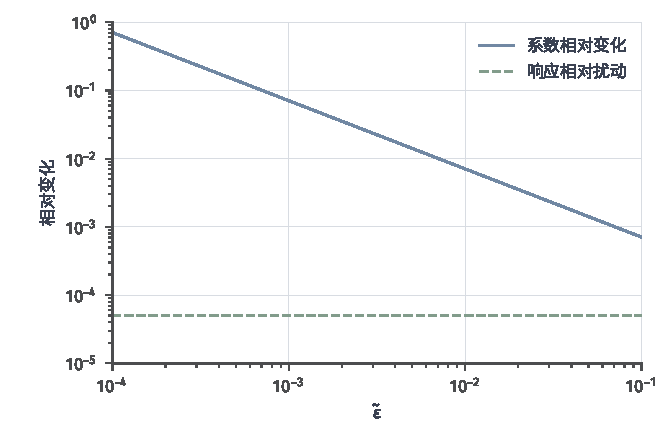
\includegraphics[width=0.92\linewidth]{figures/01-mathematical-preliminaries-upper/02-linear-spaces/matplotlib/matrix-analysis-coefficient-sensitivity/figure.pdf}
 \caption{共线设计的系数分裂：固定右端扰动 $\eta$，$\varepsilon$ 越小，两个系数
 沿相反方向偏离 $(2,0)$ 越远，绝对误差随 $1/\varepsilon$ 增长。}
 \label{fig:matrix-analysis-coefficient-sensitivity}
\end{figure}

\paragraph{拟合值和残差的变化}

系数矩阵固定时，拟合值增量
$\Delta(\bm P_{\operatorname{range}\bm A}\bm b)
=\bm P_{\operatorname{range}\bm A}\Delta\bm b$，投影不放大长度，
$\lVert\Delta\text{拟合}\rVert\leq\lVert\Delta\bm b\rVert$；残差增量落在
$(\operatorname{range}\bm A)^\perp$ 内。对新观测 $\bm a$ 的预测误差为
$\bm a^\top\Delta\hat{\bm x}$，仍受弱方向支配。

\paragraph{固定秩下的伪逆扰动}

$\bm A,\bm B=\bm A+\bm E$ 同为秩 $r$，正奇异值都不小于 $s_0>0$。有限差分恒等式
\[
 \bm B^\dagger-\bm A^\dagger
 =-\bm B^\dagger\bm E\bm A^\dagger
 +\bm B^\dagger(\bm I-\bm A\bm A^\dagger)
 -(\bm I-\bm B^\dagger\bm B)\bm A^\dagger
\]
由 Penrose 条件（\ref{thm:matrix-analysis-pseudoinverse-minimum-norm}）直接
验证；三项分别是主项与补空间耦合。在分离条件下，
\begin{equation}
 \lVert\bm B^\dagger-\bm A^\dagger\rVert
 \leq\frac{3\lVert\bm E\rVert}{s_0^2}.
 \label{eq:ch06-pseudoinverse-fixed-rank-perturbation}
\end{equation}
非主项的界来自 $\ker\bm B$ 与 $(\operatorname{range}\bm A)^\perp$ 的夹角：
对 $\bm u\in(\operatorname{range}\bm A)^\perp$，
$\lVert\bm P_{\ker\bm B}\bm u\rVert=\lVert\bm E\bm u\rVert/s_0$。

\paragraph{正奇异值的分离条件}

$\lVert\bm E\rVert<\sigma_r(\bm A)$ 只排除原方向被完全破坏，不足以保证秩不变：
零方向可能被扰动抬出一个任意小的正奇异值。式~\eqref{eq:ch06-pseudoinverse-fixed-rank-perturbation}
要求双方正奇异值都被 $s_0$ 压住，谱值分离由\ref{sec:ls-spectral-value-sensitivity}的
Weyl 界保证。

\paragraph{秩变化处的不连续性}

$\bm A=\operatorname{diag}(1,0)$，$\bm B_\varepsilon=\operatorname{diag}(1,\varepsilon)$
秩均改变：$\bm A^\dagger=\operatorname{diag}(1,0)$，而
$\bm B_\varepsilon^\dagger=\operatorname{diag}(1,1/\varepsilon)$，
$\varepsilon\to0$ 时不收敛到 $\bm A^\dagger$。秩边界上伪逆无连续界。

\subsubsection{正则化估计}
\label{sec:ls-regularized-estimate-sensitivity}

\paragraph{不稳定方向与正则化过滤}

普通伪逆按 $1/\sigma_i$ 放大噪声；截断SVD保留 $\sigma_i>\tau$ 的方向，
岭回归把增益压成滤波器 $\sigma_i/(\sigma_i^2+\lambda)$
（\ref{eq:matrix-analysis-ridge-filter-factor}，定义与目标在\ref{sec:ls-regularized-ls}）。
二者都主动削弱小奇异方向，代价是损失对应信号。

\paragraph{截断阈值的变化与跳变}

截断阈值 $\tau$ 穿过某个奇异值时，算子突然增删一个方向，估计量发生跳变；
阈值不是连续参数，选择要对照噪声水平而非拟合误差。

\paragraph{岭估计的连续收缩}

$\sigma_i^2+\lambda\geq2\sigma_i\sqrt\lambda$，故岭增益
$\sigma_i/(\sigma_i^2+\lambda)\leq1/(2\sqrt\lambda)$，增益有上界、连续变化；
拟合收缩因子 $\sigma_i^2/(\sigma_i^2+\lambda)<1$ 同时压低信号，这是偏差来源。

\paragraph{偏差和噪声放大的分解}

把 $\bm x_\lambda$ 沿SVD方向写成信号部分与噪声部分：信号被
$\sigma_i^2/(\sigma_i^2+\lambda)$ 收缩形成\term{偏差}（bias），噪声被
$\sigma_i/(\sigma_i^2+\lambda)$ 放大形成噪声项；$\lambda$ 增大两者此消彼长。
零奇异方向在普通伪逆与岭估计中都给出零，不恢复任何信息。

\paragraph{参数尺度与保留信息}

$\lambda$ 与 $\tau$ 的数值依赖特征单位：重新缩放某列后，同样的滤波强度对应
不同方向。比较不同设计的参数值没有意义，保留的信号比例才是共同口径。

\paragraph{一般惩罚算子的扰动}

一般 $\bm L$（差分惩罚等）与 $\bm A$ 不共享奇异方向，不能照搬SVD滤波器；
目标化为增广系统 $\begin{bmatrix}\bm A\\ \sqrt\lambda\,\bm L\end{bmatrix}$ 的
最小二乘，正规方程为 $(\bm A^\top\bm A+\lambda\bm L^\top\bm L)\bm x=\bm A^\top\bm y$，
公共零空间 $\ker\bm A\cap\ker\bm L$ 条件（\ref{eq:linear-algebra-tikhonov-common-nullspace}）
决定唯一性，扰动不改变该空间时解的结构稳定。可算例：$\bm A=\bm I_2$、
$\bm L=[1\ -1]$、$\bm y=(1,0)^\top$、$\lambda=1/2$，正规方程解得
$\bm x_\lambda=(3/4,1/4)^\top$——平均水平 $(x_1+x_2)/2=1/2$ 保持，相邻差由 $1$
缩为 $1/2$；而 $\bm L=\bm I$ 的岭回归给出 $(2/3,0)^\top$，不保持原平均水平，
说明一般 $\bm L$ 压缩的是自己指定的方向，不能逐方向套用岭滤波器。

\paragraph{噪声尺度误差与参数敏感度}

差异原则（\ref{eq:ls-discrepancy-constrained}）按噪声尺度 $\delta$ 选 $\lambda$：
$R(\lambda)$ 单调不增、$P(\lambda)$ 单调不减（\ref{sec:ls-method-selection}），
$\delta$ 的估计误差直接转化为 $\lambda$ 偏差；$\delta$ 低于最小可达残差时约束
恒松弛，$\delta$ 过大则退回普通最小二乘。本节只写参数对噪声尺度的敏感度，
不复述差异原则的定义与二分算法。

\subsection{谱值与子空间的敏感度}
\label{sec:ls-spectral-sensitivity}
\label{sec:linear-algebra-spectral-stability}
\label{sec:ch06-spectral-stability}

\subsubsection{谱值}
\label{sec:ls-spectral-value-sensitivity}

\paragraph{实对称特征值的有序比较}

实对称矩阵（\ref{thm:ls-real-symmetric-spectral}）的特征值全为实数，按降序排列
$\lambda_1\geq\cdots\geq\lambda_d$；扰动后 $\widetilde\lambda_1\geq\cdots\geq\widetilde\lambda_d$，
按同一次序逐个比较，不允许重新配对。

\paragraph{极值刻画与Weyl界}

Courant--Fischer 极值刻画由 Rayleigh 商（\ref{def:matrix-analysis-rayleigh-quotient}）
在子空间约束上取极小极大给出。取 $\bm A$ 的前 $k$ 维顶部子空间，$\bm E$ 在任意单位向量上的二次型
不超过 $\lVert\bm E\rVert_2$，故 $\widetilde\lambda_k\geq\lambda_k-\lVert\bm E\rVert_2$；
对称地用底部子空间得 $\widetilde\lambda_k\leq\lambda_k+\lVert\bm E\rVert_2$。

\begin{theorem}[Weyl特征值扰动界]
\label{thm:ls-weyl-eigenvalue}
对实对称 $\bm A,\bm E\in\mathbb R^{d\times d}$，按降序配对的特征值满足
\begin{equation}
 |\widetilde\lambda_k-\lambda_k|
 \leq\lVert\bm E\rVert_2,
 \qquad k=1,\dots,d.
 \label{eq:matrix-analysis-weyl-eigenvalue-perturbation}
\end{equation}
\end{theorem}

\begin{proof}
$\bm A+\bm E$ 的第 $k$ 大特征值是 $k$ 维子空间上 Rayleigh 商的极小极大。在
$\bm A$ 前 $k$ 个特征向量张成的子空间内，
$\bm x^\top(\bm A+\bm E)\bm x\geq\lambda_k\lVert\bm x\rVert^2-\lVert\bm E\rVert_2\lVert\bm x\rVert^2$，
给出下界；$\bm A$ 后 $d-k+1$ 维子空间给出上界。两式合起来即
~\eqref{eq:matrix-analysis-weyl-eigenvalue-perturbation}。
\end{proof}
该界不需要谱隙，孤立与重合的特征值都适用。

\paragraph{奇异值的绝对扰动界}

把 $\bm A\in\mathbb R^{m\times n}$ 嵌入对称分块矩阵
$\mathcal H(\bm A)=\begin{smallmatrix}\bm0&\bm A\\\bm A^\top&\bm0\end{smallmatrix}$，
其特征值为 $\pm\sigma_i$（\ref{thm:ls-svd-existence}）。$\mathcal H(\bm E)$ 的
谱范数等于 $\lVert\bm E\rVert_2$，对 $\mathcal H(\bm A)$ 与 $\mathcal H(\bm E)$
用 Weyl 界，得
\begin{equation}
 |\widetilde\sigma_i-\sigma_i|\leq\lVert\bm E\rVert_2.
 \label{eq:matrix-analysis-singular-value-perturbation}
\end{equation}
谱值读数本身稳定，不需要谱隙。

\paragraph{实可对角化矩阵的特征坐标}

实可对角化条件（\ref{sec:ls-matrix-powers}）下
$\bm A=\bm V\Lambda\bm V^{-1}$，
$\mu$ 是 $\bm A+\bm E$ 的特征值、$\bm w$ 为对应特征向量。由
$(\bm A+\bm E)\bm w=\mu\bm w$，左乘 $\bm V^{-1}$ 并整理，
\[
 (\Lambda-\mu\bm I)\bm V^{-1}\bm w
 =-\bm V^{-1}\bm E\bm w.
\]

\paragraph{特征基条件数与Bauer--Fike型界}

取离 $\mu$ 最近的 $\lambda_k$，左侧除以 $|\mu-\lambda_k|$，取范数得
\[
 |\mu-\lambda_k|
 \leq\lVert\bm V\rVert_2\lVert\bm V^{-1}\rVert_2\lVert\bm E\rVert_2
 =\kappa_2(\bm V)\lVert\bm E\rVert_2.
\]
特征向量基越病态（$\kappa_2(\bm V)$ 越大），特征值扰动界越宽；这与对称情形
$\bm V$ 正交、$\kappa_2(\bm V)=1$ 形成对照。

\paragraph{非正规性与实谱范围的限制}

非正规矩阵不能照搬对称 Weyl 界。例子 $\bm A=\begin{smallmatrix}0&1\\0&0\end{smallmatrix}$
幂零，特征值全为 $0$；左下角加 $\varepsilon$ 后
$\bm A+\bm E=\begin{smallmatrix}0&1\\\varepsilon&0\end{smallmatrix}$，
特征值为 $\pm\sqrt\varepsilon$，扰动是 $O(\sqrt\varepsilon)$ 而非 $O(\varepsilon)$；
$\varepsilon<0$ 时根本没有实特征值。非正规性使实谱对小扰动的响应失去线性
尺度。

\subsubsection{子空间}
\label{sec:ls-subspace-sensitivity}

\paragraph{基的旋转与子空间不变}

同一子空间的基可以旋转、取负号，单个基向量的变化不能直接当作子空间误差；
重特征值对应的整簇方向内部怎么转都不改变子空间。比较对象必须是子空间本身，
而不是某一组基向量。

\paragraph{主夹角的几何定义}

两个子空间的几何距离由主夹角度量，它对基的旋转与取负号都不变。

\begin{definition}[主夹角]
\label{def:matrix-analysis-principal-angles}
设 $\bm Q,\widetilde{\bm Q}\in\mathbb R^{d\times r}$ 列规范正交，分别张成 $r$ 维
子空间。交叉Gram矩阵 $\bm Q^\top\widetilde{\bm Q}$ 的奇异值为
$\cos\theta_1,\dots,\cos\theta_r$，其中 $0\leq\theta_1\leq\cdots\leq\theta_r\leq\pi/2$，
这些 $\theta_i$ 是两个子空间的\term{主夹角}（principal angles）。
\end{definition}

\paragraph{交叉Gram矩阵与主夹角计算}

对 $\bm Q^\top\widetilde{\bm Q}$ 作SVD，奇异值即 $\cos\theta_i$，配对的主方向
$\bm a_i$（取自 $\operatorname{range}\bm Q$）与 $\bm b_i$（取自
$\operatorname{range}\widetilde{\bm Q}$）满足
$\bm b_i=\cos\theta_i\,\bm a_i+\sin\theta_i\,\bm c_i$，
$\bm c_i\perp\bm a_i$。基换为 $\bm Q\bm R$、$\widetilde{\bm Q}\widetilde{\bm R}$
（$\bm R$ 正交）后，交叉矩阵右乘正交因子，奇异值不变，故主夹角与基的选择无关。

\paragraph{投影差与基无关的误差}

正交投影 $\bm P=\bm Q\bm Q^\top$、$\widetilde{\bm P}=\widetilde{\bm Q}\widetilde{\bm Q}^\top$。
用主夹角把 $2\times2$ 块写成 $\begin{smallmatrix}\cos\theta&\sin\theta\\-\sin\theta&\cos\theta\end{smallmatrix}$，
直接计算得
\[
 \lVert\bm P-\widetilde{\bm P}\rVert_2=\sin\theta_r,
 \qquad
 \frac12\lVert\bm P-\widetilde{\bm P}\rVert_{\mathrm F}^2
 =\sum_{i=1}^r\sin^2\theta_i.
\]
投影差是基无关的子空间误差度量。

\paragraph{谱隙、残差与子空间变化}

孤立特征方向的 Davis--Kahan 型界：$\bm A$ 对称，$\lambda_k$ 与其余谱的分离量为
$\gamma=\min_{j\neq k}|\lambda_j-\lambda_k|$，$\bm q$ 是单位近似特征方向，
残差 $\rho=\lVert\bm A\bm q-\mu\bm q\rVert$，则
\begin{equation}
 \sin\angle(\bm q,\bm q_k)
 \leq\frac{\lVert\bm E\rVert_2+\rho}{\gamma}.
 \label{eq:matrix-analysis-eigenvector-gap-bound}
\end{equation}
分离量 $\gamma$ 出现在分母：谱隙越小，方向对扰动越敏感。二维例子
$\bm A_\alpha=\operatorname{diag}(\alpha,-\alpha)$（两特征值相距 $2\alpha$），
$\bm E_\varepsilon=\varepsilon\begin{smallmatrix}0&1\\1&0\end{smallmatrix}$，
扰动后最大特征方向转过
$\theta=\tfrac12\arctan(\varepsilon/\alpha)\approx\varepsilon/(2\alpha)$，
图~\ref{fig:matrix-analysis-gap-direction}给出几何。整簇比较时，分离量取目标簇
与簇外最近谱值的单边距离，簇内特征值不需要彼此分开。

\begin{figure}
 \centering
 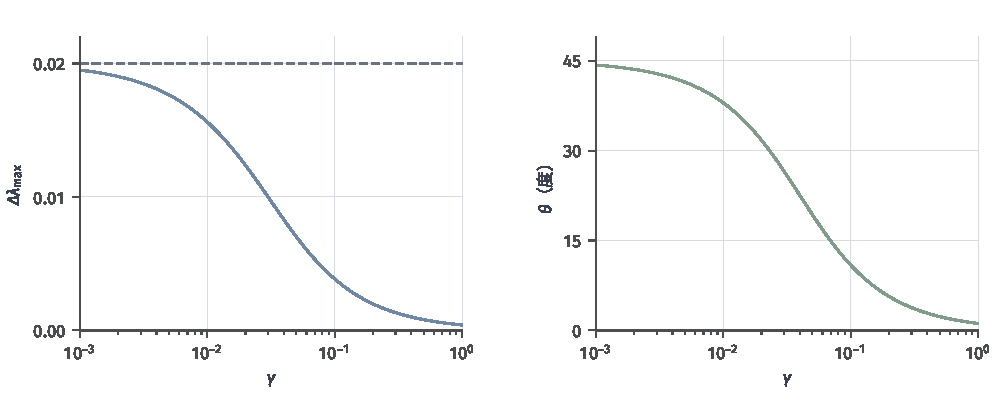
\includegraphics[width=0.92\linewidth]{figures/01-mathematical-preliminaries-upper/02-linear-spaces/matplotlib/matrix-analysis-gap-direction/figure.pdf}
 \caption{谱隙方向示意：$\bm A_\alpha$ 的两个特征值相距 $2\alpha$（谱隙），
 交叉扰动 $\varepsilon$ 把最大特征方向转过约 $\varepsilon/(2\alpha)$；
 谱隙越小，同样扰动转过的角度越大。}
 \label{fig:matrix-analysis-gap-direction}
\end{figure}

\paragraph{重特征值的整簇比较}

$\bm A=\operatorname{diag}(2,2,0)$ 中重特征值 $2$ 的平面内任意单位向量都是
特征方向，单独比较某个向量没有意义；应比较整个二维子空间。$\lambda\bm I$ 的
特征空间全空间，任何方向都不可区分，单方向误差天然无穷。

\paragraph{左右奇异子空间与Wedin型界}

对秩 $r$ 的 $\bm A$ 与 $\bm B=\bm A+\bm E$，记左、右目标子空间投影，残差为
$\lVert(\bm I-\widetilde{\bm U}\widetilde{\bm U}^\top)\bm A\rVert$ 与
$\lVert\bm A(\bm I-\widetilde{\bm V}\widetilde{\bm V}^\top)\rVert$。Wedin 型界把残差、
谱隙与子空间夹角连起来：
\begin{equation}
 \sin\theta\leq\frac{\sqrt{2r}\,\lVert\bm E\rVert_2}{\operatorname{sep}_{\mathrm W}},
 \label{eq:matrix-analysis-singular-subspace-gap}
\end{equation}
$\operatorname{sep}_{\mathrm W}$ 是目标奇异值与簇外最近奇异值的分离量；
$\sqrt{2r}$ 是粗化常数，精确块矩阵论证见\scite{math-golub2013matrix}。

\subsubsection{结构逼近}
\label{sec:ls-structured-approximation-sensitivity}

\paragraph{低秩重构与主方向的不同输出}

最佳秩 $k$ 逼近的误差由 $\sigma_{k+1}$ 控制（\ref{thm:ls-best-low-rank}），
谱值读数稳定；但逼近用到的主方向是否稳定，要看截断处是否存在谱隙，二者不是
同一个输出。

\paragraph{谱值误差与方向误差的组合}

截断SVD $\bm A_k$ 的矩阵误差同时包含谱值误差（Weyl 界）与子空间误差
（Davis--Kahan/Wedin 界）：谱值项逐项被 $\lVert\bm E\rVert$ 控制，方向项除以
分离量，后者在谱隙消失时主导。

\paragraph{截断边界和谱簇选择}

截断线穿过重复或成簇的奇异值时，边界方向对扰动敏感；此时报告整簇张成的子空间，
不单独宣称某一个主方向。选择簇边界的依据是谱值间距与噪声水平，不是拟合误差
单独决定。

\paragraph{非唯一逼近的连续性边界}

谱范数意义下最佳秩 $k$ 逼近在奇异值重复时可不唯一；Frobenius 口径由SVD唯一达到。
接近重复奇异值时，解的选择随扰动跳变，连续性只在选定口径与唯一区讨论。

\paragraph{正交逼近中的秩与选解}

极分解规范因子 $\bm Q=\bm U\bm V^\top$（\ref{def:matrix-analysis-polar-decomposition}）
在秩亏处的正交延拓不唯一；与\ref{sec:ls-ordinary-ls-sensitivity}的伪逆同理，
延拓边界上不追求连续单方向。

\subsection{矩阵函数的敏感度}
\label{sec:ls-matrix-function-sensitivity}
\label{sec:linear-algebra-matrix-function-stability}
\label{sec:ch06-matrix-function-stability}

\subsubsection{幂与指数}
\label{sec:ls-powers-exponential-sensitivity}

\paragraph{有限幂差的望远镜展开}

$(\bm A+\bm E)^k-\bm A^k$ 按乘积位置逐次插入 $\bm E$，精确展开为
\[
 (\bm A+\bm E)^k-\bm A^k
 =\sum_{j=0}^{k-1}(\bm A+\bm E)^{k-1-j}\bm E\bm A^j.
\]
每一项在固定位置插入一个 $\bm E$，这是有限增量的恒等式。

\paragraph{扰动插入位置与非交换乘法}

$k=2$ 时 $(\bm A+\bm E)^2-\bm A^2=\bm A\bm E+\bm E\bm A+\bm E^2$；
$\bm A\bm E$ 与 $\bm E\bm A$ 一般不相等，插入左侧与右侧不能合并，这是非交换性
带来的额外项，标量情形才退化为 $2\bm A\bm E$。

\paragraph{各位置传播与范数界}

取 $M=\max\{\lVert\bm A\rVert,\lVert\bm A+\bm E\rVert\}$，每一项范数不超过
$M^{k-1}\lVert\bm E\rVert$，共 $k$ 项，故
\[
 \lVert(\bm A+\bm E)^k-\bm A^k\rVert
 \leq kM^{k-1}\lVert\bm E\rVert.
\]
界随固定阶数 $k$ 线性增长，$k$ 本身进入常数。

\paragraph{矩阵指数的逐幂增量}

$\bm e^{\bm A}=\sum_{k=0}^\infty\bm A^k/k!$（\ref{sec:ls-matrix-exponential}），
把 $(\bm A+\bm E)^k$ 的望远镜展开逐项代入，指数差由各阶幂差贡献。

\paragraph{绝对级数控制与有限增量界}

不使用积分公式，直接用绝对级数控制：$\lVert e^{\bm B}\rVert\leq e^{\lVert\bm B\rVert}$，
结合幂差界逐项求和，得到随 $\lVert\bm A\rVert$、$\lVert\bm E\rVert$ 增长的粗界。
它只保证局部连续性，不是紧估计。

\paragraph{固定参数与长期变化的区别}

本节估计固定 $k$ 或固定参数处的一次函数响应；$\bm A^k$ 随 $k$ 增长或衰减的长期
行为是收敛分析的对象（\ref{sec:ls-convergence}）。$2\bm I$ 与 $\bm I/2$ 条件数
同为 $1$，幂却分别增长与衰减，条件数不回答长期问题。

学完多元微积分后可回读以下一阶响应材料，它不作为本节主线前提，有限增量论证已
独立成立。矩阵函数的一阶响应由 Fréchet 导数给出
\begin{equation}
 \mathrm d f_{\bm A}(\bm E)
 =\lim_{t\to0}\frac{f(\bm A+t\bm E)-f(\bm A)}{t},
 \label{eq:matrix-analysis-frechet-derivative}
\end{equation}
可对角化时它由除差函数
\begin{equation}
 f^{[1]}(\lambda_i,\lambda_j)
 =\frac{f(\lambda_i)-f(\lambda_j)}{\lambda_i-\lambda_j}
 \label{eq:matrix-analysis-frechet-divided-difference}
\end{equation}
经 $\bm V,\bm V^{-1}$ 作用得到；矩阵指数的 Fréchet 导数可写成积分
\begin{equation}
 \mathrm d\exp_{\bm A}(\bm E)
 =\int_0^1 e^{s\bm A}\bm E\,e^{(1-s)\bm A}\,\mathrm ds.
 \label{eq:matrix-analysis-exponential-frechet-derivative}
\end{equation}

\subsubsection{平方根与对数}
\label{sec:ls-square-root-log-sensitivity}

\paragraph{同一分支上的平方根差}

$\bm A\succ0$，正定平方根 $\bm S\succ0$ 满足 $\bm S^2=\bm A$；$\bm B=\bm A+\bm E$
仍正定，取同一正分支 $\widehat{\bm S}\succ0$，$\widehat{\bm S}^2=\bm B$。另一分支
$-\bm S$ 残差同为零，必须先选定正分支。

\paragraph{Sylvester差方程的推导}

记 $\bm D=\widehat{\bm S}-\bm S$，由
$\widehat{\bm S}^2-\bm S^2=\widehat{\bm S}\bm D+\bm D\bm S=\bm E$，
这正是以 $\widehat{\bm S},\bm S$ 为系数的Sylvester方程（\ref{def:matrix-analysis-sylvester-equation}）；
一阶近似为 $\bm S\bm Z+\bm Z\bm S=\bm E$。不能写成 $2\bm S\bm Z=\bm E$，
因为 $\bm S$ 与 $\bm Z$ 一般不交换。

\paragraph{最小特征值与平方根响应}

$\bm S$ 的本征基下，$(s_i+s_j)Z_{i,j}=E_{i,j}$，故
$\lVert\bm Z\rVert_{\mathrm F}\leq\lVert\bm E\rVert_{\mathrm F}/(2s_{\min})$，
$s_{\min}=\sqrt{\lambda_{\min}(\bm A)}$。例子 $\bm S=\operatorname{diag}(1,2)$，
$\bm E$ 的非对角元 $e$ 给出 $Z_{1,2}=e/(1+2)=e/3$，而不是 $e/2$。

\paragraph{正定对数的定义域保持}

$\log\bm A$ 只对正定矩阵定义（\ref{sec:ls-matrix-functions}）；扰动保持正定的
余量由 $\lambda_{\min}(\bm A)$ 决定，边界处先失去定义域，再谈对数误差。

\paragraph{接近零谱方向的对数放大}

对数沿 $\lambda$ 方向的响应为 $1/\lambda$，$\lambda_{\min}\to0$ 时无界；半正定
边界上对数不连续，与平方根的有界响应形成对照。

\paragraph{函数残差与分支核验}

记 $\bm R=\widehat{\bm S}^2-\bm A$，精确差方程
$\widehat{\bm S}\bm D+\bm D\bm S=\bm R$，故
$\lVert\bm D\rVert_{\mathrm F}
\leq\lVert\bm R\rVert_{\mathrm F}/(\lambda_{\min}(\widehat{\bm S})+\sqrt{\lambda_{\min}(\bm A)})$。
核验分支：残差小不区分 $\pm\bm S$，需另查正定性；$\log\det\bm A$ 是标量行列式
读数，与矩阵对数 $\log\bm A$ 不是同一对象。

\subsection{数值算法的稳定性}
\label{sec:ls-numerical-stability}

\subsubsection{数据误差与计算误差}
\label{sec:ls-data-computation-error}
\label{sec:linear-algebra-error-propagation}
\label{sec:ch06-error-propagation}

\paragraph{数据误差与计算误差的分解}

实际计算结果 $\widehat{\bm y}$ 与理想答案的差拆成两段：
\[
 \widehat{\bm y}-F(\bm z)
 =\underbrace{[\widehat{\bm y}-F(\bm z+\Delta\bm z)]}_{\text{算法计算误差}}
 +\underbrace{[F(\bm z+\Delta\bm z)-F(\bm z)]}_{\text{数据扰动误差}}.
\]
前者由算法在机器上的执行产生，后者由输入本身的误差经条件数放大，二者归因不同。

\paragraph{精确解与实际计算结果}

\term{前向误差}（forward error）即 $\widehat{\bm y}-F(\bm z)$，是最终直接测量的
误差；它同时受问题条件与算法质量影响，不能单独归给其中一方。

\paragraph{后向误差的允许集合}

\term{后向误差}（backward error）寻找最小的输入扰动 $\Delta\bm z$，使 $\widehat{\bm y}$
恰好是 $F(\bm z+\Delta\bm z)$ 的精确解。允许集合由任务规定：只允许右端改变，
或同时允许矩阵改变并保持对称；在集合内取范数最小的扰动作为后向误差度量。

\paragraph{舍入误差的局部积累}

机器实数每次运算满足浮点模型
\begin{equation}
 \operatorname{fl}(x\circ y)=(x\circ y)(1+\delta),
 \qquad |\delta|\leq u,
 \label{eq:ch06-floating-point-model}
\end{equation}
双精度 $u=2^{-53}\approx1.1\times10^{-16}$。$n$ 步运算的局部舍入累计常数为
$\gamma_n=nu/(1-nu)$，步骤越多累计越大；抵消与放大还会在中间步引入额外相对误差。

\paragraph{条件数连接后向与前向误差}

前向误差由后向误差经条件数放大：
\[
 \frac{\lVert\widehat{\bm y}-F(\bm z)\rVert}
      {\lVert F(\bm z)\rVert}
 \lesssim\kappa\cdot\frac{\lVert\Delta\bm z\rVert}{\lVert\bm z\rVert}.
\]
后向误差衡量算法把答案安放到了哪个邻近问题上，条件数再决定这个邻近问题拉开多远。

\begin{definition}[后向稳定]
\label{def:matrix-analysis-backward-stability}
算法对所有合法输入给出的结果，都是某个邻近输入的精确解，且后向误差以机器精度
$u$ 乘以与规模无关的常数为界，则称算法\term{后向稳定}（backward stable）。
\end{definition}

\paragraph{稳定算法与病态问题的区别}

后向稳定只保证 $\widehat{\bm y}$ 是邻近问题的精确解，不保证 $\widehat{\bm y}$
接近 $F(\bm z)$：病态问题（$\kappa$ 大）中，很小的后向误差经放大仍得到远离理想
答案的前向误差。稳定算法不能治愈问题本身的病态。

\subsubsection{分解与求解}
\label{sec:ls-factorization-solve}

\paragraph{计算因子与邻近矩阵}

向后误差分析把实际分解写成邻近矩阵的精确分解：算出的 $\widehat{\bm L},\widehat{\bm U}$
满足 $\widehat{\bm L}\widehat{\bm U}=\bm A+\Delta\bm A$，$\lVert\Delta\bm A\rVert$
以 $cu\lVert\bm A\rVert$ 为界，$c$ 是规模温和的误差常数。

\paragraph{消元主元增长与误差常数}

Gaussian 消元的误差常数含主元增长因子；部分选主元把增长控制在实用范围，但不
改变问题条件数。增长因子是算法实现的局部量，与 $\kappa(\bm A)$ 分别估计。

\paragraph{Cholesky的正定结构边界}

Cholesky 成功分解要求矩阵正定（\ref{sec:ls-direct-methods}）；接近半正定时代数
上仍正定但数值上可能失败，失败本身不区分“真的奇异”与“余量不足”。加对角常数
改变的是任务，不能当作修复。

\paragraph{QR和SVD的误差解释}

Householder QR 的计算因子后向正交，后向误差以 $cu$ 为界；经典Gram--Schmidt 会
逐步丢失正交性，后向界更宽。SVD 直接在 $\bm A$ 上工作，避免形成 Gram 矩阵，
子空间与伪逆由分解直接读出。

\paragraph{正规方程的条件数平方效应}

形成 $\bm A^\top\bm A$ 把条件数平方：
\begin{equation}
 \kappa_2(\bm A^\top\bm A)=\kappa_2(\bm A)^2.
 \label{eq:matrix-analysis-normal-equation-condition-square}
\end{equation}
共线例子 $\bm X_\varepsilon=
\left[\begin{smallmatrix}1&1\\0&\varepsilon\end{smallmatrix}\right]$
（见\ref{sec:ls-ordinary-ls-sensitivity}），$\kappa_2(\bm X_\varepsilon)\approx2/\varepsilon$，
而 $\bm X_\varepsilon^\top\bm X_\varepsilon=
\left[\begin{smallmatrix}1&1\\1&1+\varepsilon^2\end{smallmatrix}\right]$
的小特征值约为 $\varepsilon^2$，正规方程条件数约 $4/\varepsilon^2$；
$\varepsilon^2$ 尺度的方向在浮点中直接与零不可区分，信息先于求解损失。

\paragraph{问题病态与实现稳定性的分工}

表~\ref{tab:matrix-analysis-solver-conditions}把各路径的主要误差来源与条件数
角色并列；迭代法的残差与误差区别、收敛速率属\ref{sec:ls-convergence}，此处只
记录稳定性分工。

\begin{table}
\centering
\small
\setlength{\tabcolsep}{5pt}
\caption{直接法与迭代法的稳定性分工：条件数放大问题本身的误差，实现常数控制算法
局部误差，二者不可互相替代。}
\label{tab:matrix-analysis-solver-conditions}
\begin{tabular}{llll}
方法 & 主要误差来源 & 条件数角色 & 可靠输出 \\
\hline
带主元LU & 主元增长、回代 & 放大解误差 & 良态一般矩阵 \\
QR & 正交变换后向误差 & 不平方 & 近共线最小二乘 \\
Cholesky & 正定余量 & 放大解误差 & 正定且余量充足 \\
SVD与伪逆 & 分解本身 & 给出子空间 & 秩未知、需要选解 \\
共轭梯度 & 能量范数残差 & 决定迭代步数 & 正定对称（收敛见\ref{sec:ls-convergence}） \\
GMRES & 残差最小化 & 决定迭代步数 & 一般非对称（收敛见\ref{sec:ls-convergence}） \\
\end{tabular}
\end{table}

\subsubsection{结果核验}
\label{sec:ls-result-verification}
\label{sec:matrix-analysis-error-verification}

\paragraph{原系统残差与邻近问题}

对候选解 $\widehat{\bm x}$，原系统残差
\begin{equation}
 \bm r=\bm b-\bm A\widehat{\bm x}
 \label{eq:matrix-analysis-residual}
\end{equation}
直接可算；由 $\bm A\bm x=\bm b$ 得 $\bm x-\widehat{\bm x}=\bm A^{-1}\bm r$，
残差经逆范数变成解误差。

\paragraph{小残差不等于小解误差}

相对解误差满足
\[
 \frac{\lVert\widehat{\bm x}-\bm x\rVert}{\lVert\bm x\rVert}
 \leq\kappa(\bm A)\frac{\lVert\bm r\rVert}{\lVert\bm b\rVert}.
\]
$\bm A=\operatorname{diag}(1,\varepsilon)$，$\bm b=(1,\varepsilon)^\top$，
候选 $\widehat{\bm x}=(1,0)^\top$：精确解为 $(1,1)^\top$，残差 $\bm r=(0,\varepsilon)^\top$，
绝对残差范数为 $\varepsilon$，相对残差 $\lVert\bm r\rVert/\lVert\bm b\rVert
=\varepsilon/\sqrt{1+\varepsilon^2}\to0$，而相对解误差趋于 $1/\sqrt2$。
病态时残差小不保证解准。

\paragraph{联合扰动的归一化后向误差}

允许矩阵与右端同时改变，归一化后向误差定义为
\begin{equation}
 \eta_2(\widehat{\bm x})
 =\frac{\lVert\bm r\rVert_2}
       {\lVert\bm A\rVert_2\lVert\widehat{\bm x}\rVert_2+\lVert\bm b\rVert_2}
 \label{def:matrix-analysis-normwise-backward-error}
\end{equation}
令 $d_0=\lVert\bm A\rVert_2\lVert\widehat{\bm x}\rVert_2+\lVert\bm b\rVert_2$，
$\widehat{\bm x}\neq\bm0$ 时可取
\[
 \Delta\bm A=\frac{\lVert\bm A\rVert_2}{d_0}\,
 \frac{\bm r\,\widehat{\bm x}^\top}{\lVert\widehat{\bm x}\rVert_2},
 \qquad
 \Delta\bm b=-\frac{\lVert\bm b\rVert_2}{d_0}\,\bm r,
\]
两项分别按 $\lVert\bm A\rVert_2$、$\lVert\bm b\rVert_2$ 缩放，各自的相对尺度都
恰达到下界 $\eta_2$，且 $(\bm A+\Delta\bm A)\widehat{\bm x}=\bm b+\Delta\bm b$。
代入联合扰动界，当 $\kappa\eta_2<1$ 时解误差不超过
$2\kappa\eta_2/(1-\kappa\eta_2)$。

\paragraph{零尺度下的绝对核验}

$\bm b=\bm0$ 时分母无任意尺度，改用绝对残差；最小二乘另查正规方程残差
$\bm g=\bm A^\top\bm r=\bm0$ 与最小范数条件 $\widehat{\bm x}\perp\ker\bm A$。
例子 $\bm X=[1\ 1]$、$\bm y=2$，候选 $(3,-1)^\top$ 残差为零但非最小范数，
只有 $\bm g=0$ 与投影核验同时通过才算合格。

\paragraph{递推残差与真实残差}

迭代中递推累加的残差在几步后丢失精度，应以高精度重算 $\bm b-\bm A\widehat{\bm x}$；
递推残差用于递推，真实残差用于停止判断。

\paragraph{迭代改进与停止依据}

用同一分解解 $\bm A\bm d=\bm r_c$ 修正 $\widehat{\bm x}\leftarrow\widehat{\bm x}+\bm d$，
改进幅度受 $\kappa$ 与残差精度双重限制，数据误差到达地板后停止。停止同时核验：
真实残差、归一化后向误差与条件数估计，不以递推残差单独为准。

